\documentclass[11pt]{report}
\usepackage[utf8]{inputenc}
\usepackage[T1]{fontenc}
\usepackage[unicode=true]{hyperref}
\usepackage{lmodern}
\usepackage[french]{babel}

%%% PAGE DIMENSIONS
\usepackage{geometry}
\geometry{a4paper}
\geometry{top=2.5cm, bottom=2.5cm, left=4.5cm , right=3.5cm}
\usepackage{graphicx}


%%% PACKAGES
\usepackage{booktabs} % for much better looking tables
\usepackage{array} % for better arrays (eg matrices) in maths
\usepackage{paralist} % very flexible & customisable lists (eg. enumerate/itemize, etc.)
\usepackage{verbatim} % adds environment for commenting out blocks of text & for better verbatim
\usepackage{subfig} % make it possible to include more than one captioned figure/table in a single float
\usepackage{amssymb,amsmath}
\usepackage{xcolor}
\usepackage{sistyle}
\usepackage{shorttoc}
\usepackage{titlesec}
\usepackage{titletoc}

\hypersetup{breaklinks=true,
            pdfauthor={Thibault Deutsch (deutsc\_t); Ilan Dubois (dubois\_o); Arthur Douillard (douill\_a); Axel Mendoza (mendoz\_a)},
            pdftitle={Rapport de soutenance 1},
            colorlinks=true,
            citecolor=blue,
            urlcolor=blue,
            linkcolor=black,
            pdfborder={0 0 0}}

\setlength{\parskip}{6pt plus 2pt minus 1pt}
\setlength{\emergencystretch}{3em}  % prevent overfull lines

\setcounter{secnumdepth}{3}
\setcounter{tocdepth}{4}
\renewcommand{\thechapter}{\Roman{chapter}}
\renewcommand{\thesection}{\arabic{section}.}
\renewcommand{\thesubsection}{\arabic{section}.\arabic{subsection}}
\renewcommand{\thesubsubsection}{\arabic{section}.\arabic{subsection}.\arabic{subsubsection}}

\usepackage{fancyhdr} % This should be set AFTER setting up the page geometry
\pagestyle{fancy}
\fancyhead[L]{(Neurone)\up{*}}
\fancyhead[C]{}
\fancyhead[R]{Oh! Ça seRt}

\title{Rapport de soutenance 1}
\author{Thibault Deutsch (deutsc\_t) \and Ilan Dubois (dubois\_o) \and Arthur Douillard (douill\_a) \and Axel Mendoza (mendoz\_a)}
\date{29 octobre 2014}

\dottedcontents{chapter}%
  [\dimexpr 10mm]
  {}
  {\dimexpr 10mm}
  {3.2mm}

\dottedcontents{figure}%
  [\dimexpr 15mm]
  {}
  {\dimexpr 15mm}
  {3.2mm}

\begin{document}
\renewcommand{\labelitemi}{$\bullet$}

\begin{titlepage}
\newcommand{\HRule}{\rule{\linewidth}{0.5mm}} % Defines a new command for the horizontal lines, change thickness here

%----------------------------------------------------------------------------------------
%	LOGO SECTION
%----------------------------------------------------------------------------------------
\flushright

\includegraphics[width = 4.5cm]{epita.png}\\[0.5cm] % Include a department/university logo - this will require the graphicx package

%----------------------------------------------------------------------------------------
%	HEADING SECTIONS
%----------------------------------------------------------------------------------------
\textsc{\Large Rapport de soutenance 1}\\[0.15cm] % Major heading such as course name
\textsc{\large 2\up{ème} année du cycle préparatoire}\\[3cm] % Minor heading such as course title

%----------------------------------------------------------------------------------------
%	TITLE SECTION
%----------------------------------------------------------------------------------------
\center
\HRule \\[0.5cm]
{\Huge \bfseries Oh! Ça seRt}\\[0.3cm] % Title of your document
\textsc{\Large Un OCR dévelopé en C}\\[0.1cm]
\large Réalisé par le groupe \emph{(Neurone)\up{*}}\\[1.5cm]
\large 29 octobre 2014\\[0.1cm]
\HRule \\[2cm]


\includegraphics[width = 10cm]{logo.png}\\[1cm]

\Large
\textbf{Thibault Deutsch} (\emph{deutsc\_t}) \\
\textbf{Ilan Dubois} (\emph{dubois\_o}) \\
\textbf{Arthur Douillard} (\emph{douill\_a}) \\
\textbf{Axel Mendoza} (\emph{mendoz\_a})\\[2cm]

%----------------------------------------------------------------------------------------
\vfill % Fill the rest of the page with whitespace

\end{titlepage}

\newpage
\pagenumbering{arabic}
\shorttableofcontents{Sommaire}{1}

\chapter{Introduction}

Ce document est le rapport de soutenance 1. Son objectif est de présenter une synthèse du travail fournit par l’équipe du projet (Neurone)\up{*}.\ Ce groupe est composé de quatre étudiants en deuxième année du cycle préparatoire de l’EPITA : Thibault DEUTSCH (deutsc\_t), Ilan DUBOIS (dubois\_o),  Axel MENDOZA (mendoz\_a), et Arthur DOUILLARD (douill\_a).

Le projet consiste en la réalisation d’un logiciel de reconnaissance optique de caractères (OCR, en anglais \emph{optical character recognition}). Le but de ce logiciel est de convertir un document numérisé, à l'aide d'un scanner, en un fichier numérique modifiable. Pour cela, le programme doit être capable de reconnaître la structure du document et de reconnaître les différents caractères.

Nous devons réalisés ce projet en C. Son développement se déroule sur une période d’environ trois mois, en équipe de quatre personnes. Ce projet à pour objectifs, outre l'apprentissage du C, de nous familiariser avec le développement sur environnement GNU/Linux, le respect d'un cahier des charges, ains que le travail de groupe sur un projet commun.

Nous avons choisi d’appeler notre groupe (Neurone)\up{*} en référence à l’étoile de Kleene vu en conférence de THLR\footnote{Théorie des langages rationnels}. Le choix du nom du projet a été fait dans un objectif comique, ``Oh ça sert'' a bien sûr pour initiales OCR\footnote{Ce n'est pas immédiat, mais tout de même...}.

La répartition des tâches est présentée dans le tableau en figure~\ref{tab}.

\colorlet{darkgreen}{green!60!black}

\begin{figure}[htbp]
\centering
\begin{tabular}{ | c || c | c | c | c | }
\hline Tâches & Thibault & Ilan & Arthur & Axel \\
\hline Modélisation & & & \textcolor{darkgreen}{X} & \\
\hline Moteur graphique & \textcolor{darkgreen}{X} & & \textcolor{darkgreen}{X} & \\
\hline Moteur physique & & \textcolor{darkgreen}{X} & & \textcolor{darkgreen}{X} \\
\hline Menu & & \textcolor{darkgreen}{X} & & \textcolor{darkgreen}{X} \\
\hline Réseau & \textcolor{darkgreen}{X} & & \textcolor{darkgreen}{X} & \textcolor{darkgreen}{X} \\
\hline Gameplay & \textcolor{darkgreen}{X} & \textcolor{darkgreen}{X} & & \\
\hline Audio & & \textcolor{darkgreen}{X} & & \textcolor{darkgreen}{X} \\
\hline Site web & \textcolor{darkgreen}{X} & \textcolor{darkgreen}{X} & & \\
\hline
\end{tabular}
\caption{Répartition des tâches sur l'ensemble de la durée du projet}
\label{tab}
\end{figure}

Vous trouverez dans la suite de ce rapport une présentation détaillée sur les différentes dimensions du développement.

%\begin{figure}[htbp]
%\centering
%\includegraphics[width=8cm]{batiment.png}
%\caption{Modélisation d'un bâtiment}
%\end{figure}

\chapter{Pré-traitement}

Les filtres et masques flou, dans un logiciel à reconnaissance de caractère, sont utilisés lors du pré-traitement. Cette étape préalable à détection des caractères est indispensable. En effet, son but est d’adaptés les caractéristiques de l'image à notre algorithme qui segmentera l'image en lignes et en caractères. L'image subit alors plusieurs transformations. En premier lieu, nous devons saturé les couleurs de celle-ci afin d'obtenir uniquement du noir et du blanc. Le second traitement consiste à éliminer le bruit, grâce à l'application d'un filtre sur notre image d'origine.

\section{Filtres}

%TODO: courte intro

Après m'être documenté sur la partie de l'élimination du bruit, à l'aide de documents se réfèrent au bruit dans les images, aux différents problèmes récurrents en imagerie numérique et aux méthode utilisés pour résoudre ces problèmes. J'ai choisit deux méthodes pour éliminer le bruit, le filtre moyen qui est un filtre basique à but purement pédagogique, et le filtre gaussien qui effectue un flou plus sophistiqué et mieux adaptés à notre projet. L'image à traiter proviendra d'un scanner, nous remarquerons que cette image aura certains défauts qu'il faudra éliminer à l'aide du flou en question. En effet, si l'image est floue, le passage d'une valeur à l'autre se fait plus progressivement et l'algorithme de détection de caractères et donc plus optimale. Mathématiquement, une image est rendue floue en utilisant un filtre qui élimine les détails associés à de plus hautes fréquences qui constitue le bruit et les parasites en imagerie numérique qui polluent l'information. Malheureusement, nous ne pouvons appliquer directement un filtre passe-bas ``classique'' sur notre image car cette méthode risque de supprimer les petits caractères isolés tel que les points sur les ``i'' ou les accents. C'est pour cela que nous avons choisit d'appliquer une méthode qui adapte le flou en fonction de la nature des pixels voisins.

Nous allons aborder maintenant le principe du flou gaussien. En premier lieu, il nous faut définir l'opération mathématique appelée ``convolution'' utilisé dans tout les filtres dit linéaires. Lorsqu'il s'agit de données numérisés comme dans notre cas en traitement d'image, la relation entre les valeurs des pixels d'entrée et celle des pixels de sortie est décrite par un tableau de nombres, généralement carré, appelé matrice de convolution.  Le filtre gaussien, comme son nom l'indique, utilise la loi de probabilité de Gauss et la courbe gaussienne. Le principale problème de ce filtre est que l'application directe de la formule gaussienne nécessite un temps de calcul considérable. Heureusement, certains algorithmes effectuent ce calcul à l'aide d'approximations de plus en plus précises qui améliore grandement la complexité de l'algorithme qui applique ce filtre sur notre image.

\begin{figure}[htbp]
\centering
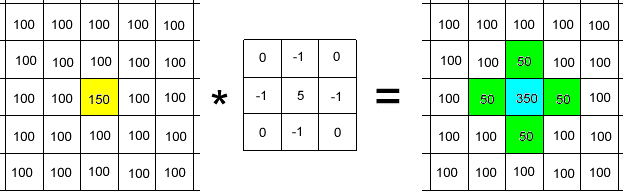
\includegraphics[width=9cm]{matconvol.jpg}
\caption{Application d'une matrice de convolution}
\end{figure}

Au départ nous avons utilisé un filtre moyen, qui calcule les composants de chaque pixels en fonctions de ses pixels directement adjacents mais nous n'étions pas convaincue en ce qui concerne  l'efficacité de ce flou. La première méthode du filtre gaussien, consiste à appliquer une matrice de convolution de dimension impaire ($3 \times 3, 5 \times 5, …$). Une matrice de convolution de dimension $3 \times 3$ nous a parut plus performant. En effet, plus la dimension de la matrice est élevée, plus la perte d'information est importante. Chaque pixels de l'image est modifié en fonction des composantes des pixels environnants. Plus la matrice de convolution est grande, plus les composantes des  pixels seront influencées par les pixels environnants. En somme, plus notre matrice de convolution est grande, plus le flou est important. En appliquant la matrice sur un pixel, les produits des composantes des pixels voisins avec la valeur de la matrice correspondante. Le résultat est en suite divisé par la somme des valeurs de notre matrice de convolution. 

\begin{figure}[htbp]
\centering
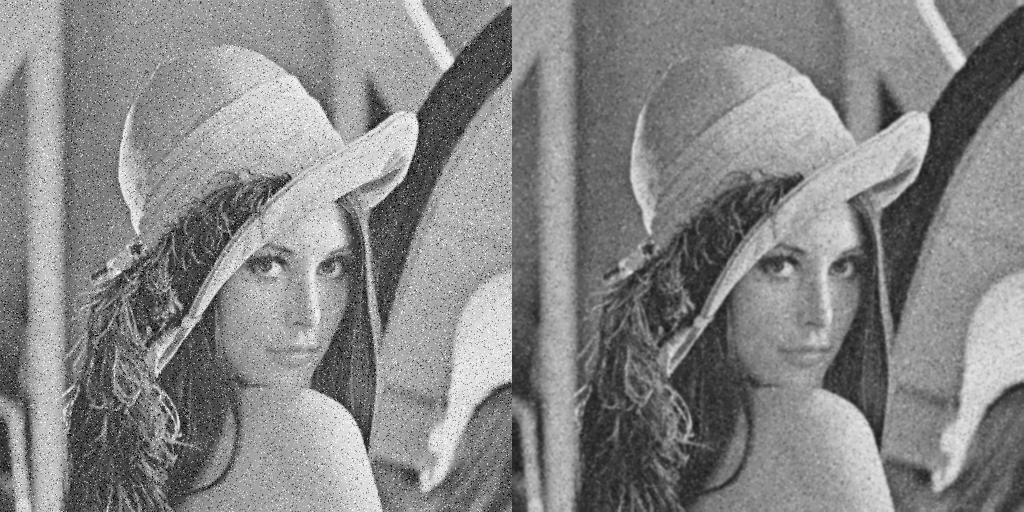
\includegraphics[width=9cm]{filtre_gaussien.png}
\caption{Application du filtre gaussien sur une image bruitée}
\end{figure}

Le principe du filtre gaussien est donc le suivant : on parcours l'image pixel par pixel, en appliquant le masque sur chaque pixels et ses voisins. On stocke le résultat des calculs effectuer sur les pixel dans une variable constituant un tableau à deux dimensions et on retourne cette variable. Nous avons également utilisé une fonction qui nous renvoi le symétrique d'un pixel par rapport à la matrice de convolution lorsque ce pixel était en dehors de notre image. Lorsque l'on veut appliquer le masque sur un pixel au bord de l'image, on tente de sommer les composantes d'un pixel qui n'existe pas. Mais lorsque l'on somme le pixel symétrique à celui-ci et qu'on le divise par le coefficient au même emplacement dans le masque, le résultat n'est pas erroné.

\chapter{Réseau de neurones}

\chapter{Site web}

\chapter{Conclusion}

Le projet Troma a débuté en janvier 2014, nous avions l'objectif de réaliser un jeu de guerre sous le thème de la Seconde Guerre Mondiale. Le groupe est formé de quatre étudiants en première année sans connaissance préalable particulière en langage C\#. Cependant nous avons décidé dès le début de donner notre maximum en choisissant un jeu en 3D muni d'un mode de jeu en ligne ! 

Durant toute la phase de développement nous avons essayé de garder cet état d'esprit qui est de toujours donner le maximum. Les notes que nous avons obtenues aux deux premières soutenances nous ont encourager à continuer dans cette voie. Nous avons donc implémenter toutes les fonctionnalités du jeu une par une avec plus ou moins de difficulté mais sans jamais abandonner même quand cela s'avérait beaucoup plus difficile que prévu. L'aspect technique n'a pas été la seule difficulté, le côté organisationnel des soutenances et du planning à respecter pour l'équipe en a aussi été une! Notre point fort a été de ne jamais attendre le dernier moment et d'essayer de prendre le maximum d'avance possible sur notre planning prévisionnel lorsque cela était possible.

Aujourd'hui nous sommes fiers d'avoir réussi à mener à bien notre projet de bout en bout. Cette expérience a été très enrichissante pour chacun d'entre nous. Nous pensons que ce travail de groupe nous permettra d'aborder avec plus de facilité nos futurs projets à l'EPITA et/ou en entreprise.

\newpage
\pagenumbering{Roman}
\part*{Annexes}

\newpage
\listoffigures

\newpage
\tableofcontents
 
\end{document}
